\section[RESTful]

Segundo Richardson, para que uma API de estilo REST seja considerada RESTful, esta deve seguir estritamente as regras exigidas anteriormente. Além disso, propõem uma escala de quatro níveis para avaliar a coesão e maturidade dessas API's. \cite{RichardsonEtAl2013}

\begin{itemize}[noitemsep]
\item \textbf{Nível 0}: É a falta de qualquer regra; diz respeito ao uso de HTTP para operações de endereços no servidor. Normalmente, usa apenas um ponto de acesso (URI) e um verbo HTTP.
\item \textbf{Nível 1}: Aplicação de recursos. A API é dividida em diferentes pontos de acesso que indicam um ou mais recursos.
\item \textbf{Nível 2}: Implementação de verbos HTTP para diferentes tipos de operações. Onde uma mesma URI pode aceitar mais de um verbo para execução de diferentes procedimentos.
\item \textbf{Nível 3}: O conceito de HATEOS é aplicado para disponibilizar informações necessárias para interação e navegação da API.
\end{itemize}

\begin{figure}[H]
  \centering
  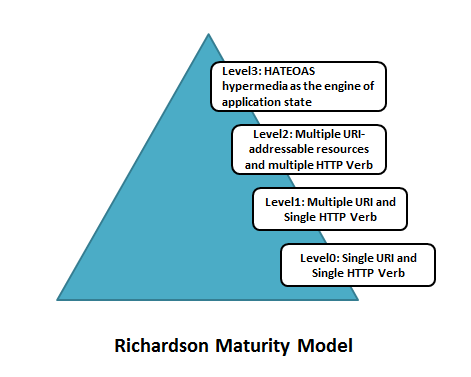
\includegraphics[width=0.75\textwidth,height=\textheight,keepaspectratio]{figuras/richardson-maturity-model.png}
  \caption{Modelo de Maturidade descrito por Richardson}
\end{figure}
